



\documentclass[12pt]{article}

\usepackage[brazil]{babel}
\usepackage[utf8]{inputenc}
\usepackage{graphicx}
\usepackage{float}
\usepackage{indentfirst}
\usepackage{cite}

\title{Análise de relacionamento em um grupo de desenvolvimento de software}
\author{
	Marcelo Gianfaldoni de Andrade\\
	Engenharia da Computação\\
	Insper\\
}
\date{\today}


\begin{document}
\maketitle

\newpage
\tableofcontents
\newpage

\begin{abstract}
Esse texto busca analisar as relações entre um grupo de desenvolvimento de software composto por programadores e administradores. Dentro da divisão dos programadores, há aqueles que preferem trabalhar em módulos produzidos por grupos separados e aqueles que preferem trabalhar em um mesmo módulo com os mesmos colegas. Serão feitas simulações de relacionamento entre os indivíduos do grupos para diferentes quantidades de cada um dos três tipos de indivíduo descrito, para no fim, entender as consequências desses casos.
\end{abstract}

\section{Introdução}
Em um grupo de desenvolvimento de software, foi-se dividido três tipos de integrantes. Os administradores, que não tem contato direto com ferramentas e linguagens de programação, os programadores que preferem integram módulos distintos feitos por grupos separados, e os programadores que preferem trabalhar em um só módulo com os mesmos colegas. O objetivo desse texto é simular e analisar esse cenário para investigar o que pode acontecer com a comunidade para diferentes distribuições de integrantes no time.

\section{Método Utilizado}
Para classificar melhor os três tipos de integrantes, usou-se uma definição mais formal do comportamento de cada um deles, sendo classificados assim, os programadores que integram módulos, os programadores que participam de um só grupo e os administradores, de respectivamente:

\begin{itemize}
	\item Openers
	\item Closers
	\item Chummy
\end{itemize}


Openers seriam os integrantes que procuram não fechar grupos, para uma definição mais formal, pode-se dizer que querem diminuir fórmula de Burt, definida em \cite{burt}. Os Closers seriam o oposto, buscam fechar grupos entre si, ou mais formalmente, diminuir o inverso da fórmula de Burt. Por fim, os Chummies querem fazer o maior número de amigos possível, ou seja, o maior número de conexões.

Quando defini-se esses três integrantes dessa maneira, é possível analisar o comportamento da comunidade através de grafos onde os nós são integrantes do time e as arestas são simplesmente a existência de uma relação entre eles.

Para de simular diferentes tipos de situações, dividiu-se as simulações em três conjuntos, nos quais não existiria nenhum integrante de cada uma das três classificações em cada conjunto. Sendo assim o primeiro onde não há Openers, o segundo onde não há Closers, e o terceiro onde não há Chummies. E para facilitar a simulação, considerou-se um time de 15 pessoas, variando a proporção de cada um dos grupos de integrantes.

Com o contexto das simulações definidas, escolheu-se algumas variáveis para analisar quantitativamente os resultados, sendo essas o número médio de arestas do grafo, o número médio de componentes, e como se comportam os valores de centralidade para cada um dos dois grupos não zerados de integrantes(se não há Closers, esses grupos seriam Chummies e Openers, por exemplo).

Em anexo pode ser encontrado os gráficos resultantes de todas as simulações feitas, mas apenas algumas serão analisadas com enfoque para uma melhor conclusão. Resultados em que os valores são todos zeros não foram colocados em anexo.

\section{Análise}

Quando se é zerado o número de closers, pode-se perceber que o número de componentes permanece em um independente da relação entre openers e chummies, como visto na figura \ref{fig7}. Isso mostra que esse time teria uma relação coesa independente da classificação dos integrantes, desde que não haja closers. Já a centralidade dos openers e chummies são relativamente proporcionais ao número de cada um deles no time, como visto na figura \ref{fig9}.

Quando se é zerado o número de Chummies, o número de componentes permanece aproximadamente um enquanto há poucos openers, como visto na figura \ref{fig2}. No entanto, com o aumento de openers, o número de componentes no grafo acaba aumentando, chegando próximo a três, sendo assim um time pouco coeso, em que há grupos não conectados. 

O padrão descrito acima aparece novamente quando é zerado o número de openers, pode-se perceber que o número de componentes fica próximo a um quando há poucos chummies, mas esse valor aumenta até aproximadamente dois quando o número de chummies aumenta, como visto na figura \ref{fig11}. Mais uma vez, o time pode ficar pouco coeso, e com grupos que não se relacionam.

Pode-se perceber também que não há valor de centralidade nos closers, independente a situação simulada, pois buscam sempre formar um grupo entre si em o número de conexões entre os integrantes do grupo são iguais.

\section{Conclusão}

Por fim, para um melhor desempenho e ambiente no time de desenvolvimento, pode-se perceber que os integrantes do time closers não são recomendados. Segundo as simulações e análises feitas anteriormente, conclui-se que um time formado por openers e chummies gera um só componente, ou seja, um grupo que se relaciona totalmente, tendo assim possivelmente um melhor resultado final de trabalho.

\section{Anexo}

%---------------------------------------------------------------------------
% Figure
%---------------------------------------------------------------------------
\begin{figure}[H]
	\centering
	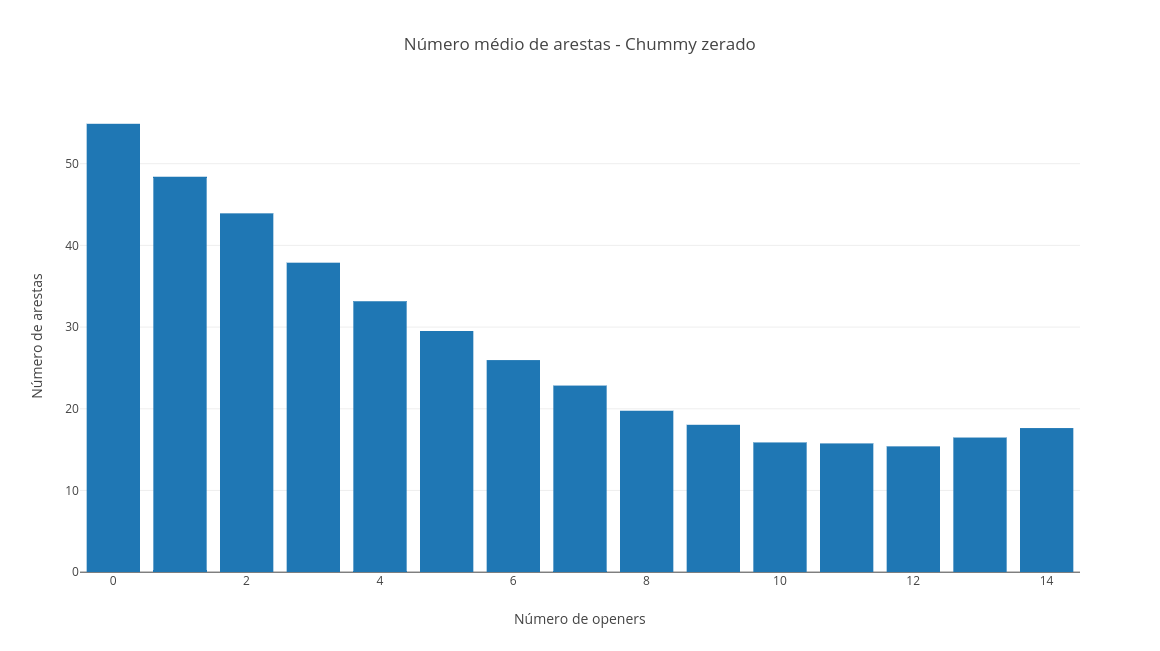
\includegraphics[width=\textwidth, height=200px]{basic-bar.png}
    \caption{Número médio de arestas - Chummy Zerado}
	\label{fig1}
\end{figure}

\begin{figure}[H]
	\centering
	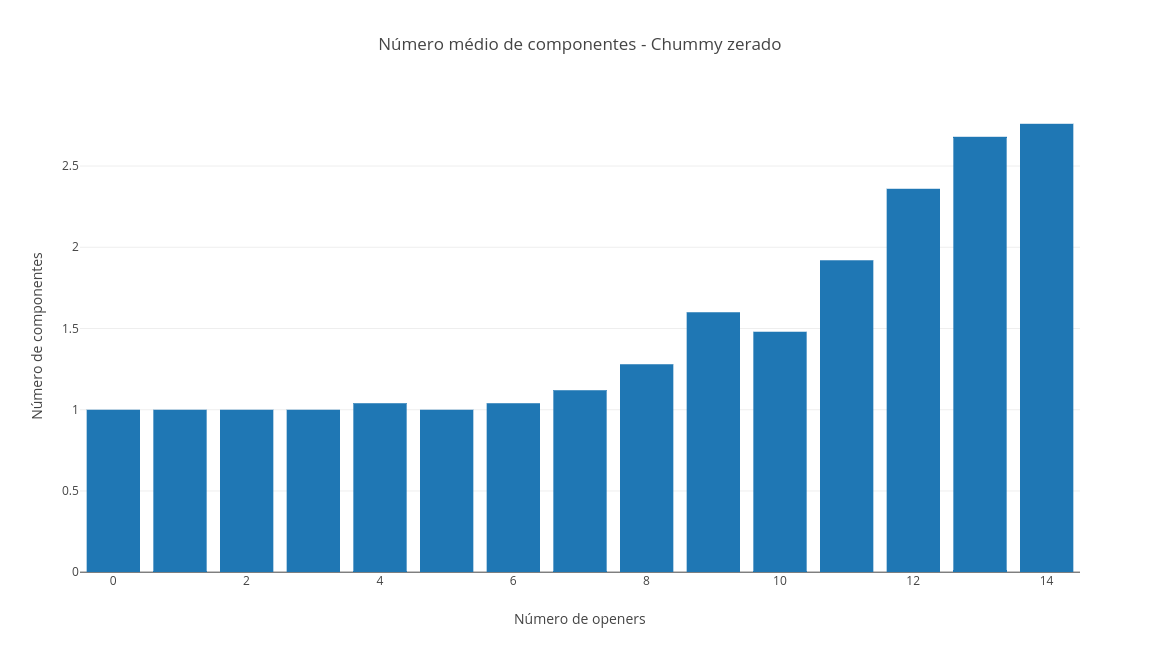
\includegraphics[width=\textwidth, height=200px]{basic-bar_2.png}
	\caption{Número médio de componentes -Chummy Zerado}
	\label{fig2}
\end{figure}

\begin{figure}[H]
	\centering
	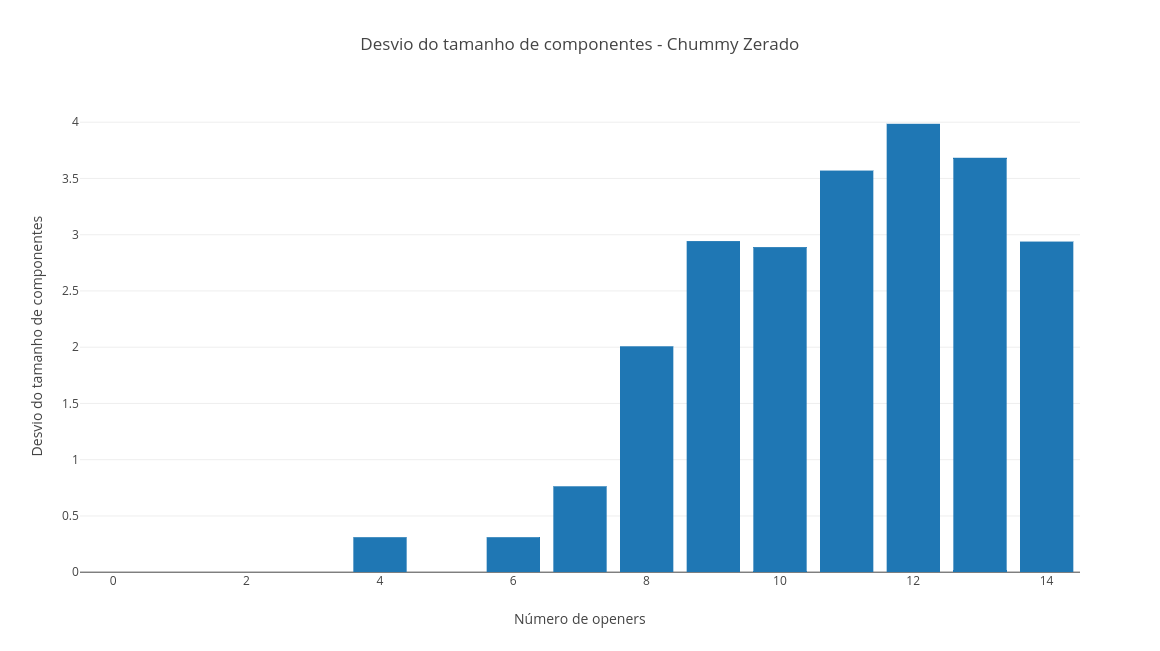
\includegraphics[width=\textwidth, height=200px]{basic-bar_3.png}
	\caption{Desvio do tamanho de componentes - Chummy Zerado}
	\label{fig3}
\end{figure}

\begin{figure}[H]
	\centering
	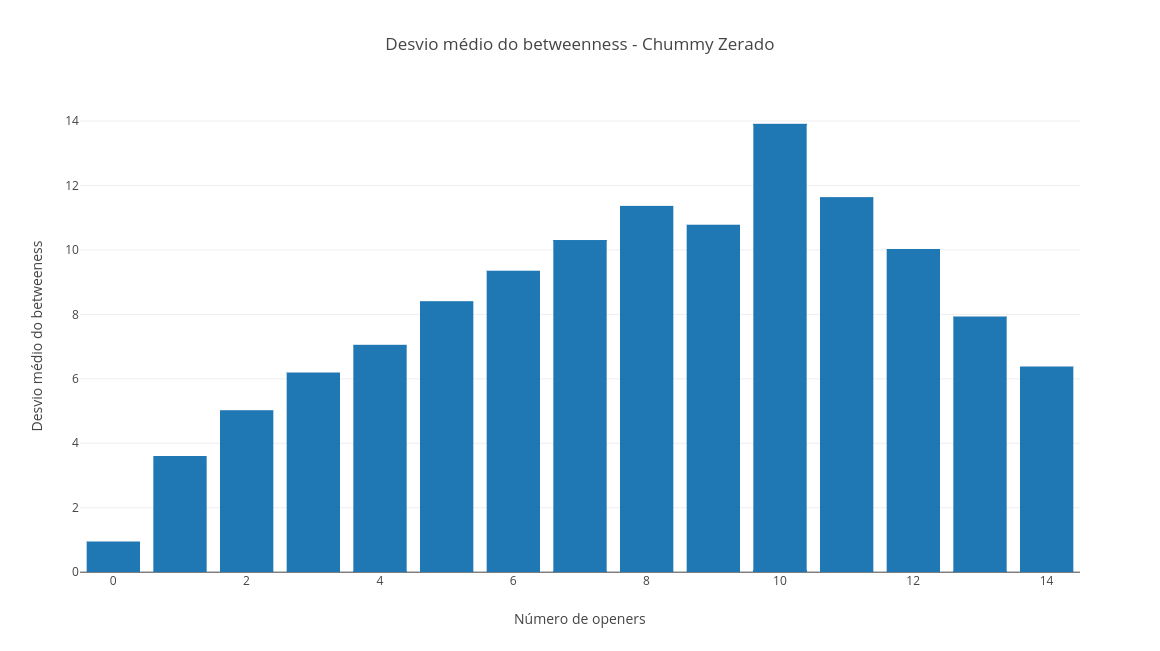
\includegraphics[width=\textwidth, height=200px]{basic-bar_4.png}
	\caption{Desvio médio do betweenness - Chummy Zerado}
	\label{fig4}
\end{figure}

\begin{figure}[H]
	\centering
	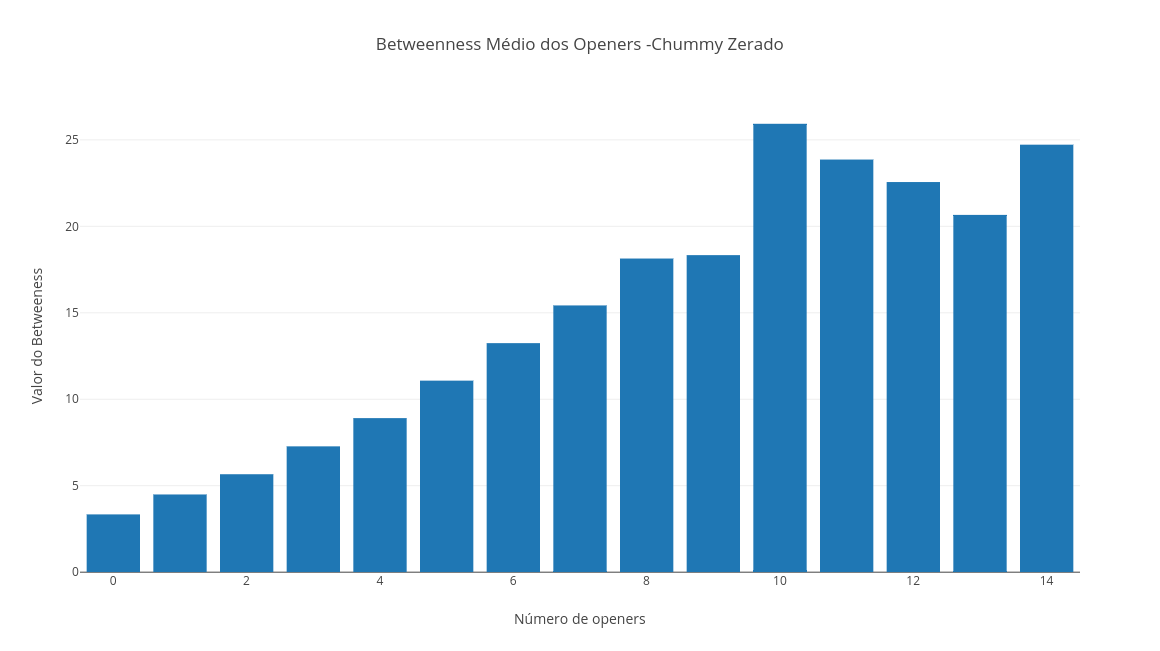
\includegraphics[width=\textwidth, height=200px]{basic-bar_5.png}
	\caption{Betweennes médio dos Openers - Chummy Zerado}
	\label{fig5}
\end{figure}

\begin{figure}[H]
	\centering
	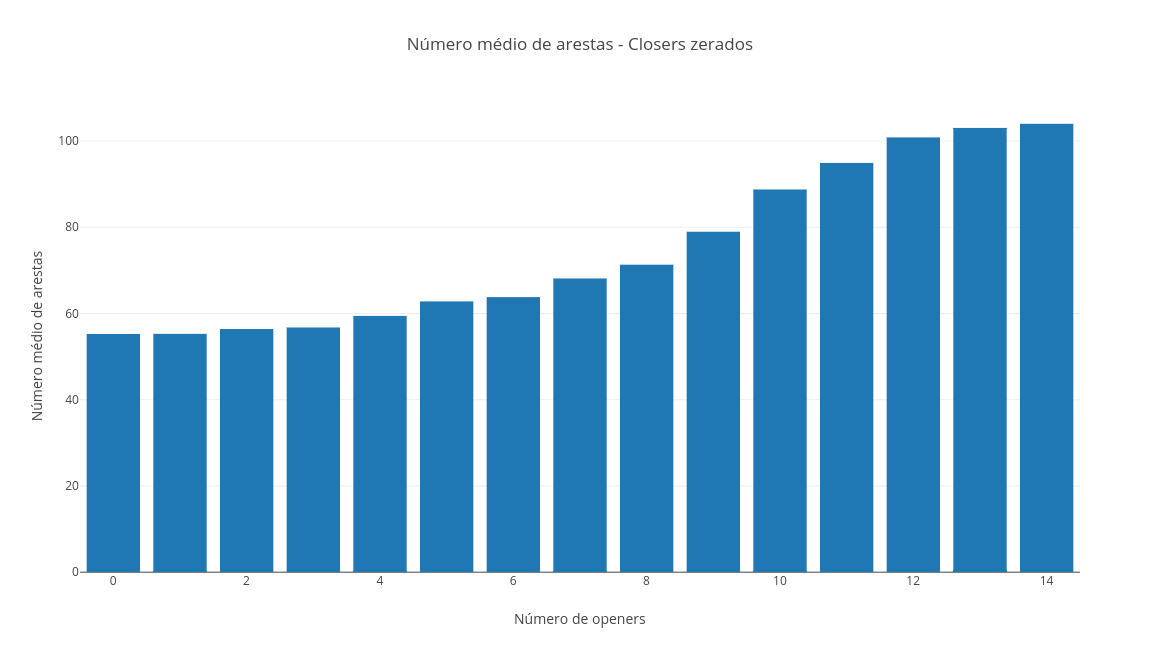
\includegraphics[width=\textwidth, height=200px]{basic-bar_6.png}
	\caption{Número médio de arestas - Closers Zerados}
	\label{fig6}
\end{figure}

\begin{figure}[H]
	\centering
	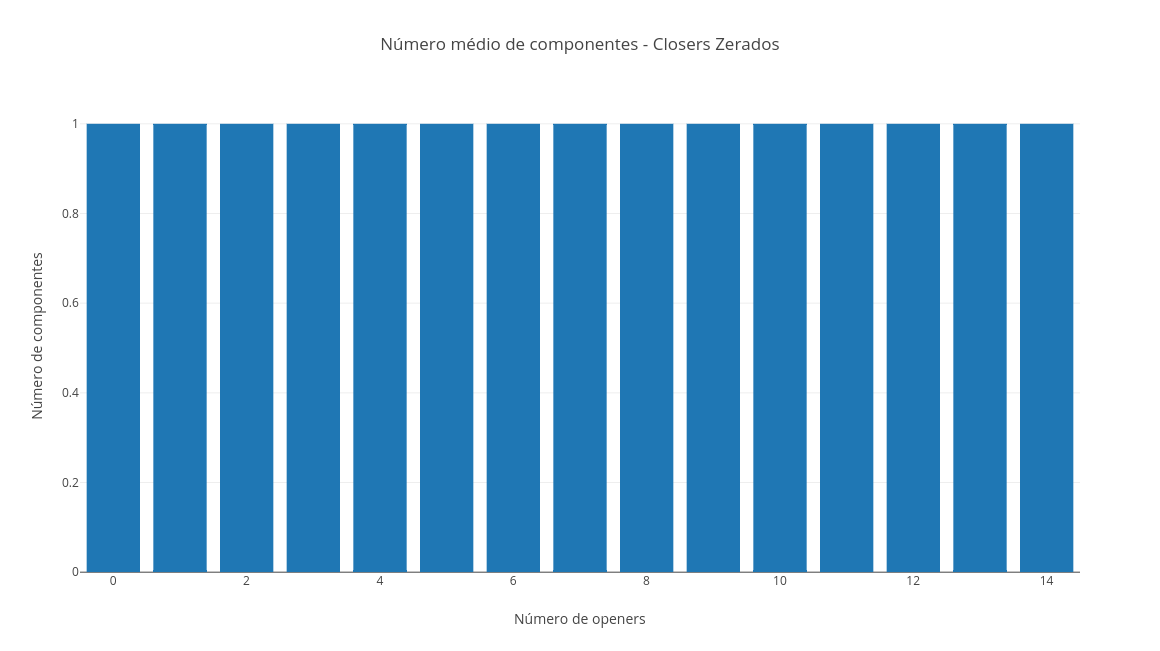
\includegraphics[width=\textwidth, height=200px]{basic-bar_7.png}
	\caption{Número médio de componentes - Closers Zerados}
	\label{fig7}
\end{figure}

\begin{figure}[H]
	\centering
	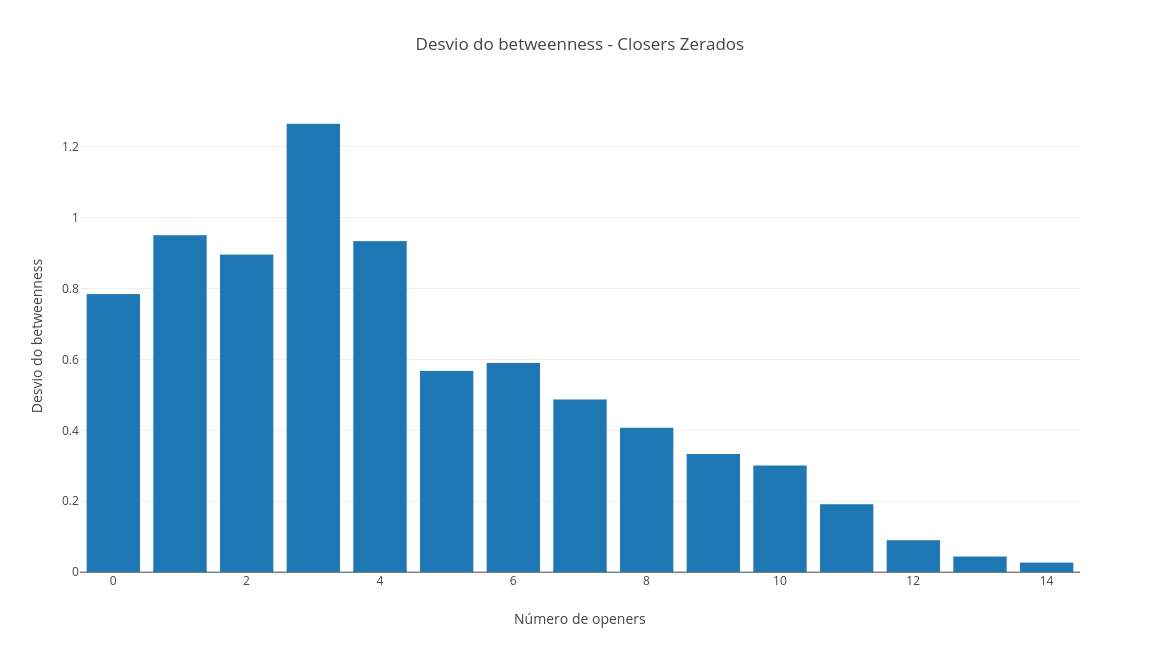
\includegraphics[width=\textwidth, height=200px]{basic-bar_8.png}
	\caption{Desvio do betweenness - Closers Zerados}
	\label{fig8}
\end{figure}

\begin{figure}[H]
	\centering
	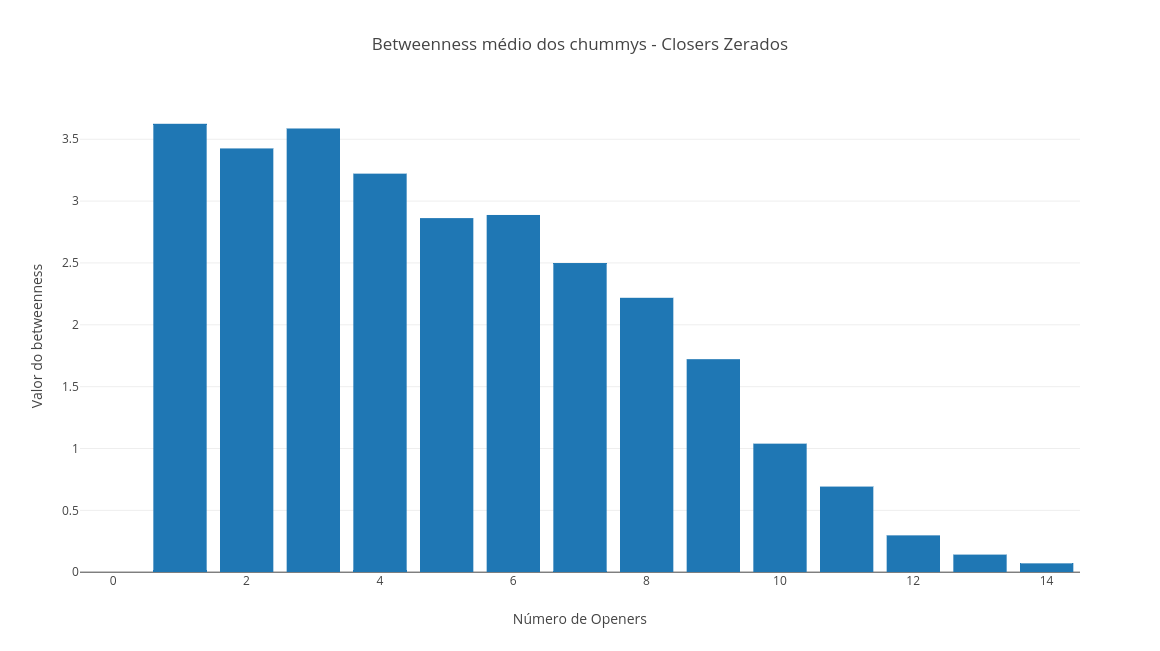
\includegraphics[width=\textwidth, height=200px]{basic-bar_9.png}
	\caption{Betweenness médio dos chummies - Closers Zerados}
	\label{fig9}
\end{figure}

\begin{figure}[H]
	\centering
	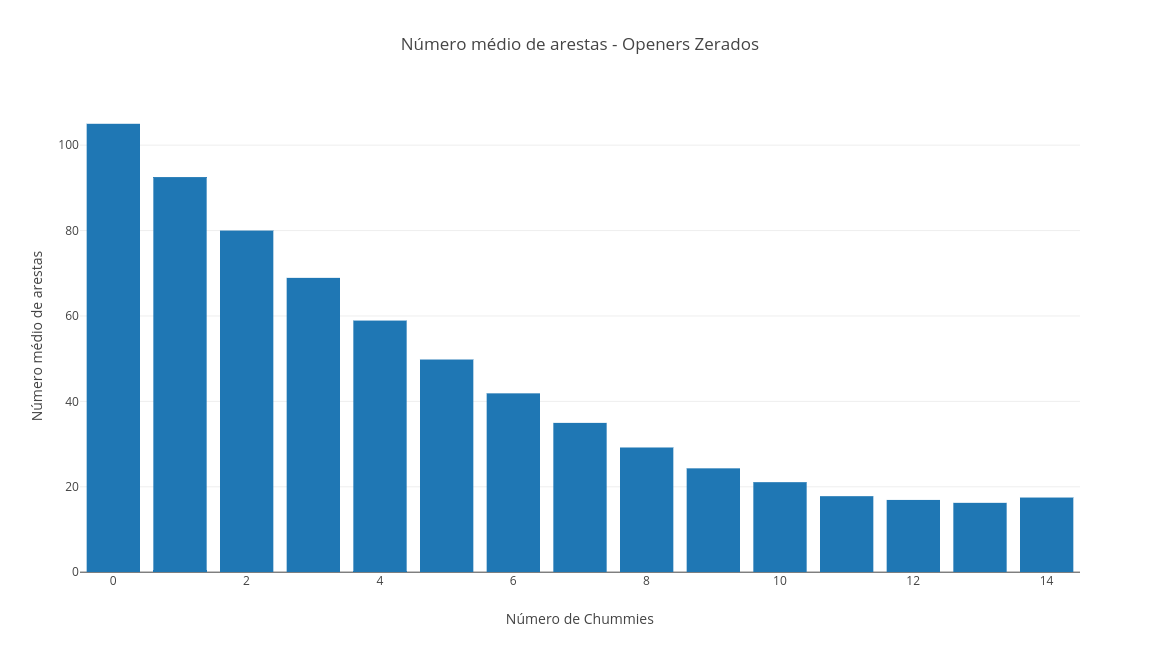
\includegraphics[width=\textwidth, height=200px]{basic-bar_11.png}
	\caption{Número médio de arestas - Openers Zerados}
	\label{fig10}
\end{figure}

\begin{figure}[H]
	\centering
	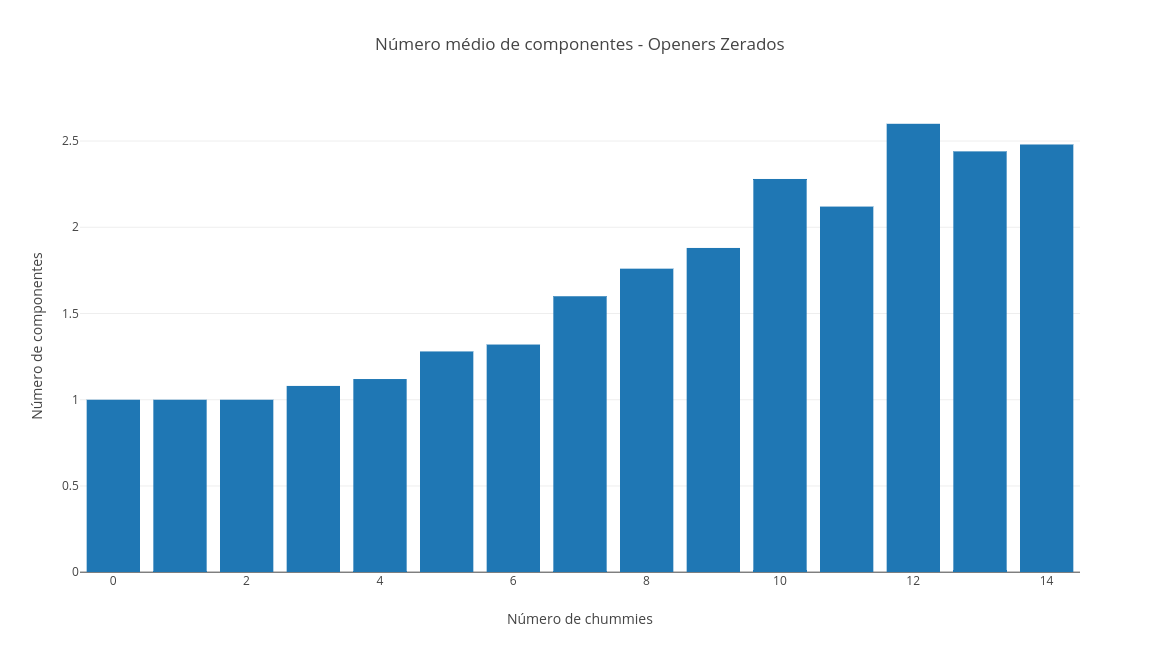
\includegraphics[width=\textwidth, height=200px]{basic-bar_12.png}
	\caption{Número médio de componentes - Openers Zerados}
	\label{fig11}
\end{figure}

\begin{figure}[H]
	\centering
	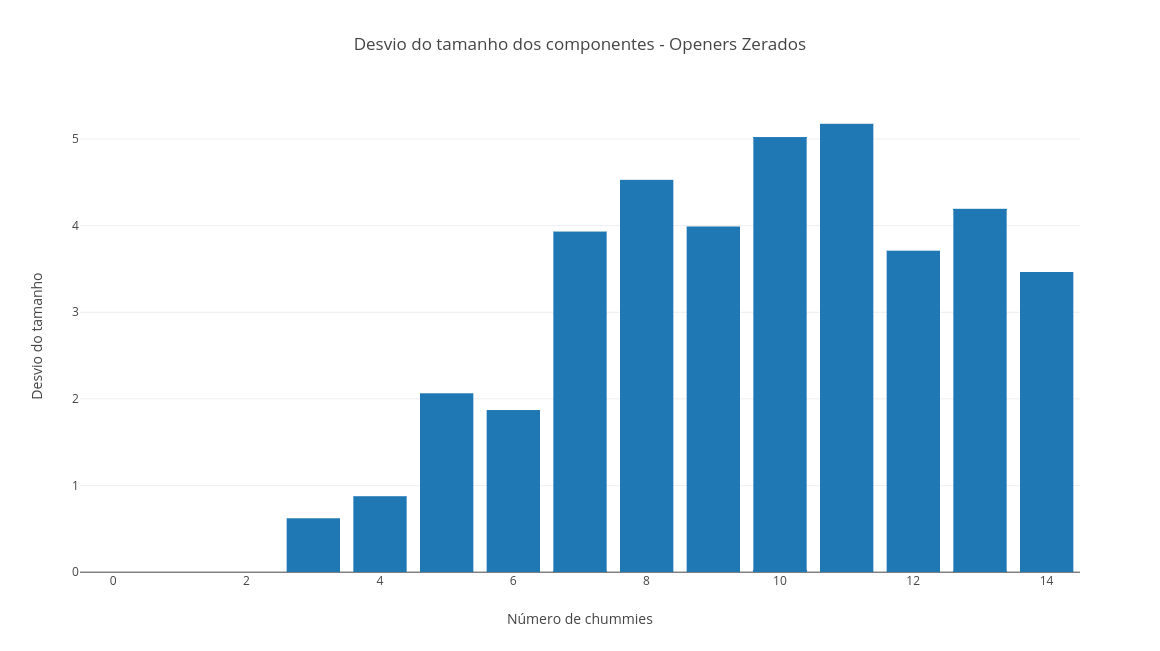
\includegraphics[width=\textwidth, height=200px]{basic-bar_13.png}
	\caption{Desvio do tamanho dos componentes - Openers Zerados}
	\label{fig12}
\end{figure}

\begin{figure}[H]
	\centering
	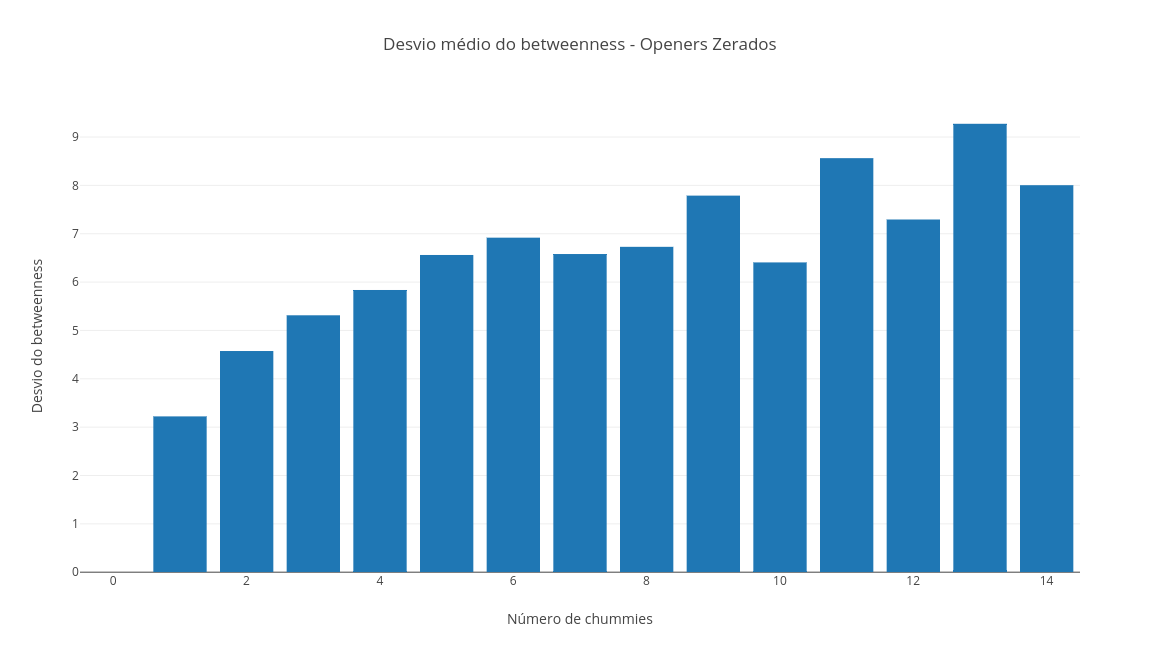
\includegraphics[width=\textwidth, height=200px]{basic-bar_14.png}
	\caption{Desvio médio do betweenness - Openers Zerados}
	\label{fig13}
\end{figure}

\begin{figure}[H]
	\centering
	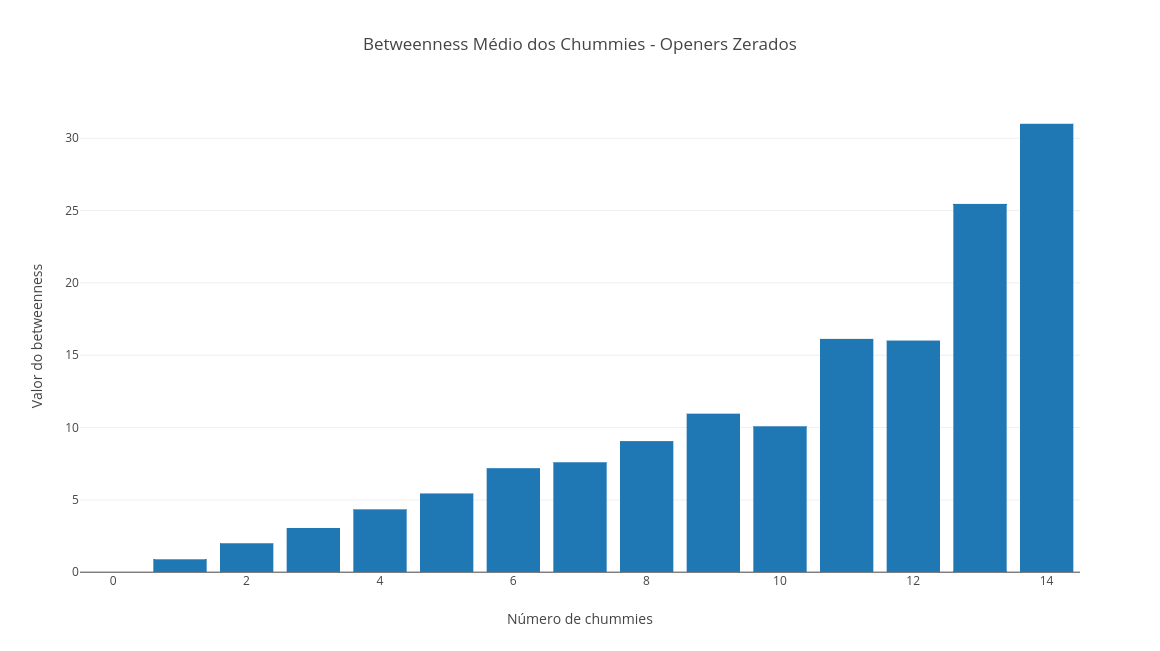
\includegraphics[width=\textwidth, height=200px]{basic-bar_15.png}
	\caption{Betweenness Médios dos Chummies - Openers Zerados}
	\label{fig14}
\end{figure}


\bibliography{bibliografia}{}
\bibliographystyle{plain}

%---------------------------------------------------------------------------

\end{document}
  